\documentclass[11pt,a4paper,oneside,openany]{report}
\usepackage{marginnote}
\usepackage{wallpaper}
\usepackage{lastpage}
\usepackage[left=1.3cm,right=4.6cm,top=1.8cm,bottom=4.0cm,marginparwidth=3.4cm]{geometry}
\usepackage{amsmath}
\usepackage{amssymb}
\usepackage{xcolor}
\usepackage{pgfplotstable} 
\usepackage{booktabs} 
\usepackage{filecontents}
\usepackage{longtable}
\usepackage{graphicx,multicol}
\usepackage[spanish]{babel}
\usepackage[utf8]{inputenc}
\usepackage{verbatim} % añadir este paquete para tener la salida correcta del txt
\usepackage{wallpaper}%para imagen de fondo
\usepackage[utf8]{inputenc}


\usepackage{subfig}

\usepackage[labelformat=empty]{caption}
 \captionsetup[figure]{labelformat=empty}
\usepackage{fancyhdr}
\setlength{\headheight}{80pt}
\pagestyle{fancy}\fancyhf{}
\renewcommand{\headrulewidth}{0pt} 
\setlength{\parindent}{0cm}
\newcommand{\tab}{\hspace*{2em}}
\newcommand\BackgroundStructure{ % Command to specify the background of each page
\setlength{\unitlength}{1mm} % Set the unit length to millimeters

%\author{Ricardo}
%\title{\LARGE Reporte Prueba \textsc{Red}}
%\date{\today}
%\ThisCenterWallPaper{1.45}{ClusterReporte1/beige.jpg}%Add background image only on this page


\setlength\fboxsep{0mm} % Adjusts the distance between the frameboxes and the borderlines
\setlength\fboxrule{0.5mm} % Increase the thickness of the border line
\put(10, 10){\fcolorbox{black}{blue!10}{\framebox(155,247){}}} % Main content box
\put(165, 10){\fcolorbox{black}{blue!10}{\framebox(37,247){}}} % Margin box
\put(10, 262){\fcolorbox{black}{white!10}{\framebox(192, 25){}}} % Header box
\put(175, 263){
\includegraphics[height=23mm,keepaspectratio]{logo1}} % Logo box - maximum height/width: 
}

%----------------------------------------------------------------------------------------
%       HEADER INFORMATION
%----------------------------------------------------------------------------------------

\fancyhead[L]{\begin{tabular}{l r | l r} % The header is a table with 4 columns
\textbf{Reporte} & Cluster Agave & \textbf{Página} & \thepage/\pageref{LastPage} \\ % Project name and page count
\textbf{Día} & \today & % Version and reviewed date
\textbf{Responsable} & Dr. Alejandro Morales \\ % Designer and reviewer
\end{tabular}}

%----------------------------------------------------------------------------------------

\AddToShipoutPicture{\BackgroundStructure} % Set the background of each page to that specified above in the header information section

%----------------------------------------------------------------------------------------
%       DOCUMENT CONTENT
%----------------------------------------------------------------------------------------

\begin{document}

 \begin{titlepage}
    \ThisCenterWallPaper{1.45}{beige.jpg}
    %\ThisULCornerWallPaper{0.7}{barra3.jpg}
	%\ThisURCornerWallPaper{0.305}{agave.jpg}
	\centering
	{\scshape\tiny . \par}
	%\vspace{0cm}
	{\huge\bf Clúster Agave \par}
	\vspace{1cm}
	
\includegraphics[width=0.7\textwidth]{udg.png}\par
	%{\scshape\Large Universidad de Guadalajara \par}
	\vspace{2.7cm}
	{\Huge\bfseries Reporte de estado \par}
	\vspace{2cm}
	{\huge \today \par}
	\vfill
	supervisado por\par
	Dr.Alejandro Morales
	\vfill
	{\Large\itshape Software de reportes hecho por Ricardo Amador Castañeda\par}
		
 \end{titlepage}

\section{Actividad de usuarios.}

\marginnote{Listado de \\usuarios y su \\correspondiente \\actividad. }

\resizebox{14cm}{!}{}

\section{Usuarios}
	{\huge Espacio  utilizado  por los usuarios}
  	\verbatiminput{espacio_usuarios.txt}
    {\huge Horas  activos}
    \verbatiminput{actividad_horas.txt}


\section{Estatus Nodos}

\marginnote{Información de los nodos inactivos.}
	{\huge Nodos Activos}
	\verbatiminput{nodesup.txt}
	{\huge Nodos Inactivos}
	\verbatiminput{nodesDown.txt}
	  

%Imagenes del cluster

\newpage
\section{detalles Nodos}
\textit{Tiempo que cada nodo lleva activo desde su ultimo apagado: }
\verbatiminput{uptime.txt}
\textit{Uso del Clúster por día en horas. (ejemplo: si un 2 usuarios usaron el Clúster \\
	    2 horas en un día, esto equivaldría a 4 horas de uso en total por el día)}
\verbatiminput{uso_dia.txt}	  
\textbf{Memoria RAM}
\verbatiminput{memoria.txt}	  

	 



\newpage

\section{Carga de trabajo y gráficos de rendimiento.}

\marginnote{Actividad del cluster por nodo. Se incluyen gráficas de rendimiento.}

%\begin{figure}[htb]
%\centering
%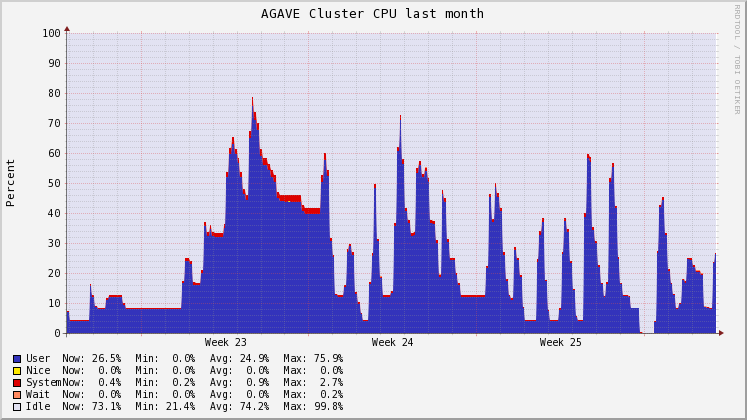
\includegraphics[width=0.9\linewidth]{porciento}\\
%\caption{Uso en porcentaje del CPU del nodo maestro}
%\end{figure}

\begin{figure}[htb]
\centering
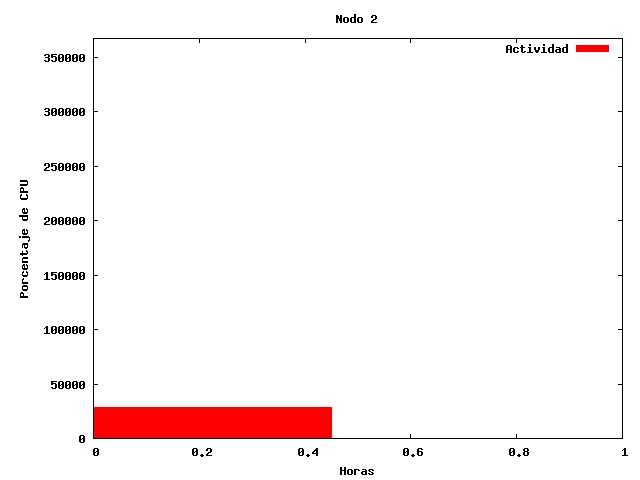
\includegraphics[width=0.9\linewidth]{memoria1.jpg}\\
\caption{Uso de memoria en Bytes durante el mes para el cluster}
\end{figure}

\begin{figure}[htb]
\centering
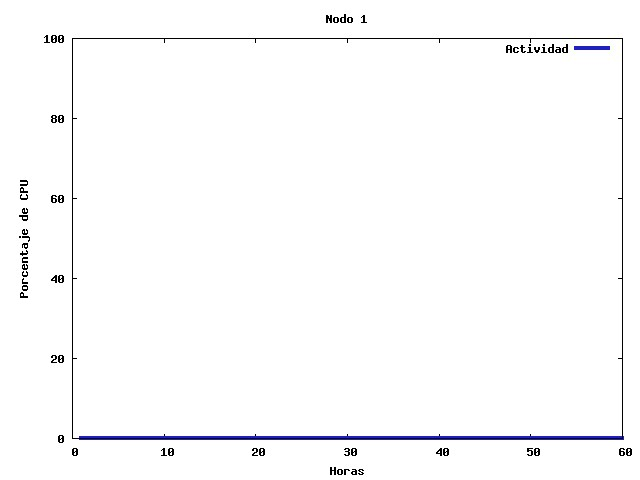
\includegraphics[width=0.9\linewidth]{grafico1.jpg}\\
\caption{Uso de procesadores del primer nodo durante el mes}
\end{figure}

\begin{figure}[htb]
\centering
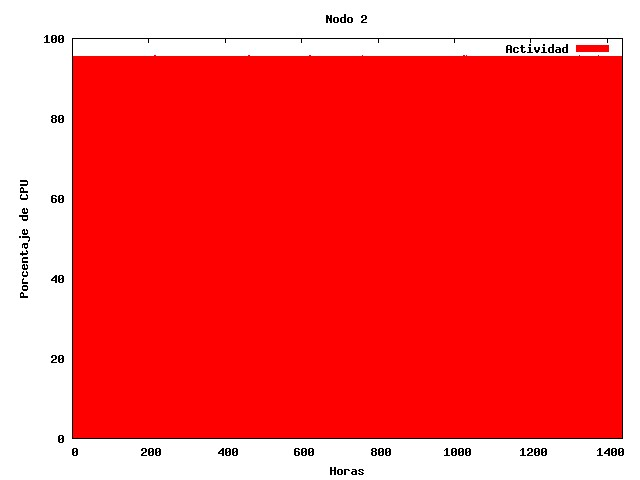
\includegraphics[width=0.9\linewidth]{grafico2.jpg}\\
\caption{Uso de procesadores del segundo nodo durante el mes}
\end{figure}


\begin{figure}[htb]
\centering
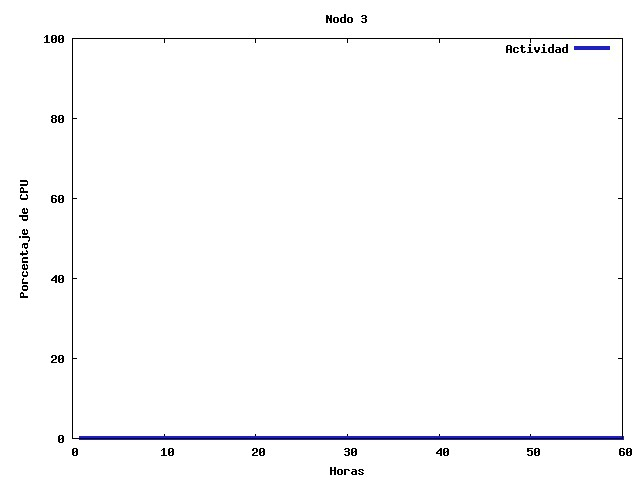
\includegraphics[width=0.9\linewidth]{grafico3.jpg}\\
\caption{Uso de procesadores del tercer nodo durante el mes}
\end{figure}

\begin{figure}[htb]
\centering
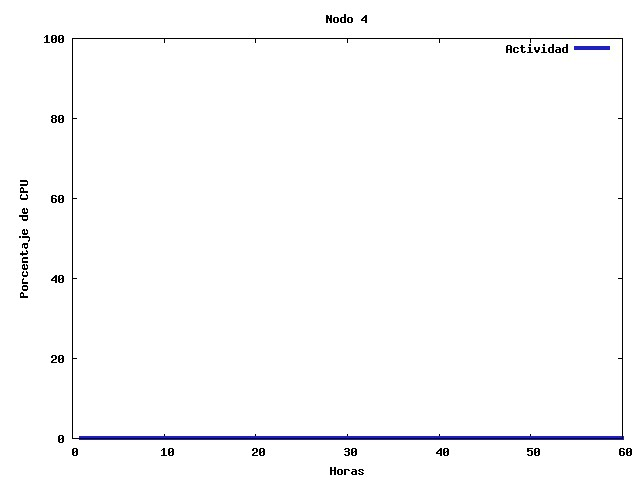
\includegraphics[width=0.9\linewidth]{grafico4.jpg}\\
\caption{Uso de procesadores del cuarto nodo durante el mes}
\end{figure}

\begin{figure}[htb]
\centering
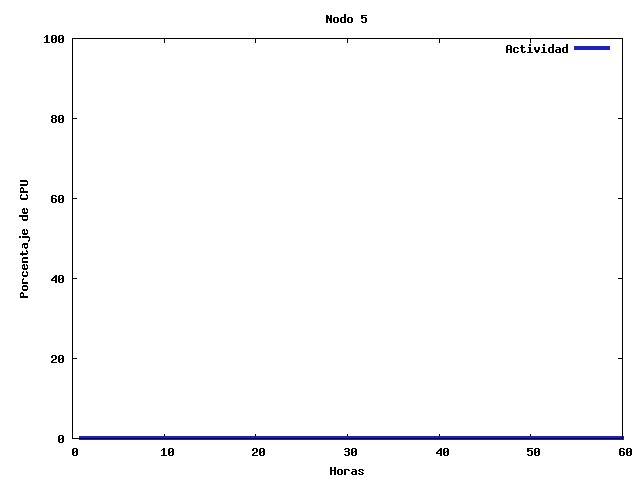
\includegraphics[width=0.9\linewidth]{grafico5.jpg}\\
\caption{Uso de procesadores del quinto nodo durante el mes}
\end{figure}

\begin{figure}[htb]
\centering
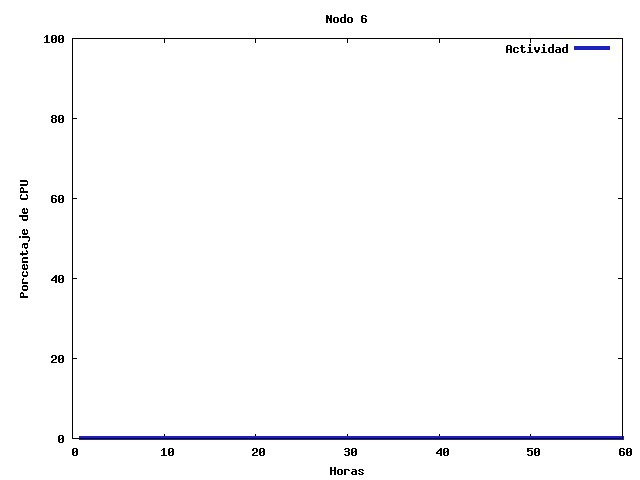
\includegraphics[width=0.9\linewidth]{grafico6.jpg}\\
\caption{Uso de procesadores del sexto nodo durante el mes}
\end{figure}

\begin{figure}[htb]
\centering
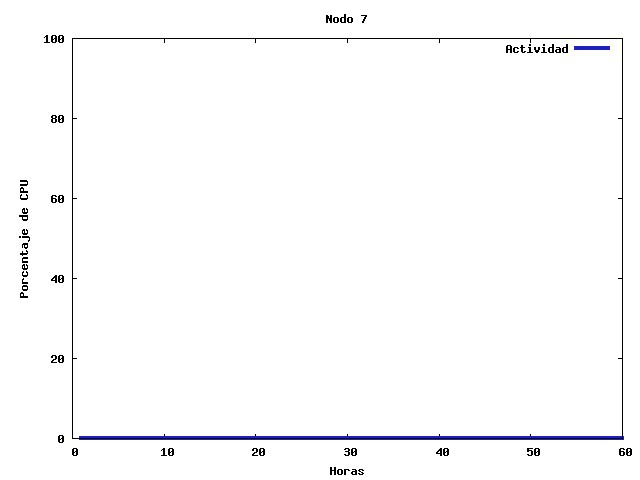
\includegraphics[width=0.9\linewidth]{grafico7.jpg}\\
\caption{Uso de procesadores del séptimo nodo durante el mes}
\end{figure}

\begin{figure}[htb]
\centering
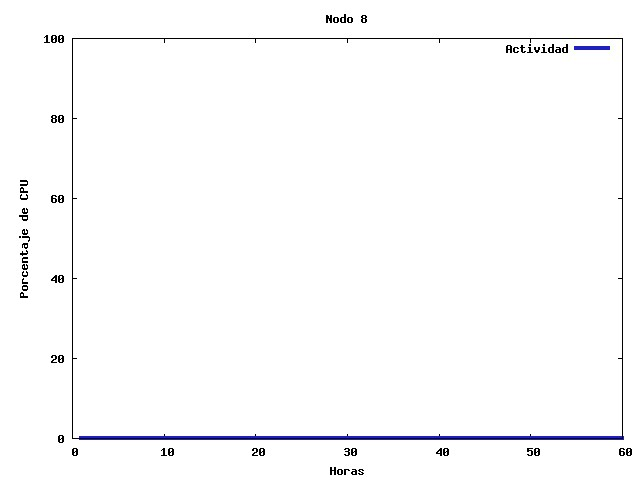
\includegraphics[width=0.9\linewidth]{grafico8.jpg}\\
\caption{Uso de procesadores del octavo nodo durante el mes}
\end{figure}

\begin{figure}[htb]
\centering
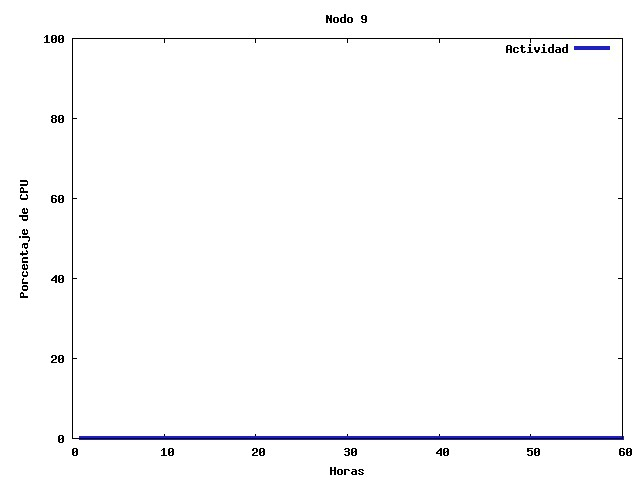
\includegraphics[width=0.9\linewidth]{grafico9.jpg}\\
\caption{Uso de procesadores del noveno nodo durante el mes}
\end{figure}

\begin{figure}[htb]
\centering
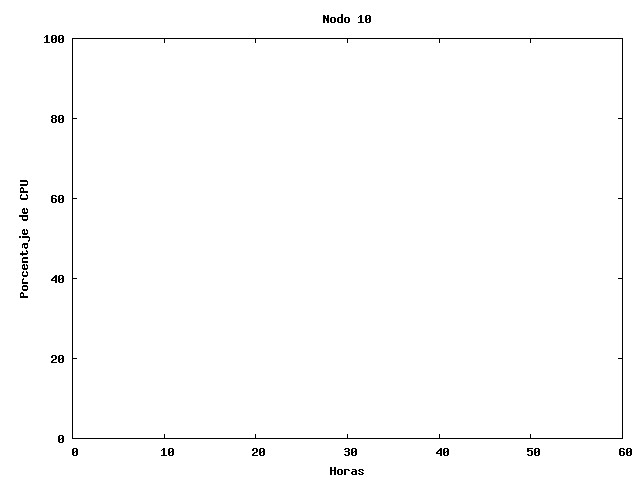
\includegraphics[width=0.9\linewidth]{grafico10.jpg}\\
\caption{Uso de procesadores del decimo nodo durante el mes}
\end{figure}

\begin{figure}[htb]
\centering
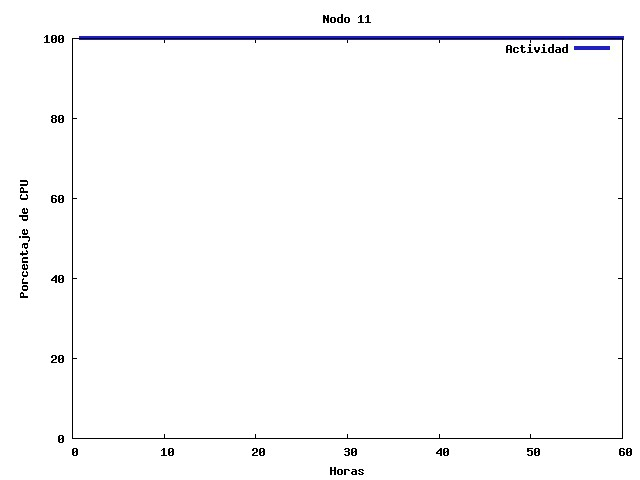
\includegraphics[width=0.9\linewidth]{grafico11.jpg}\\
\caption{Uso de procesadores del undécimo nodo durante el mes}
\end{figure}

\begin{figure}[htb]
\centering
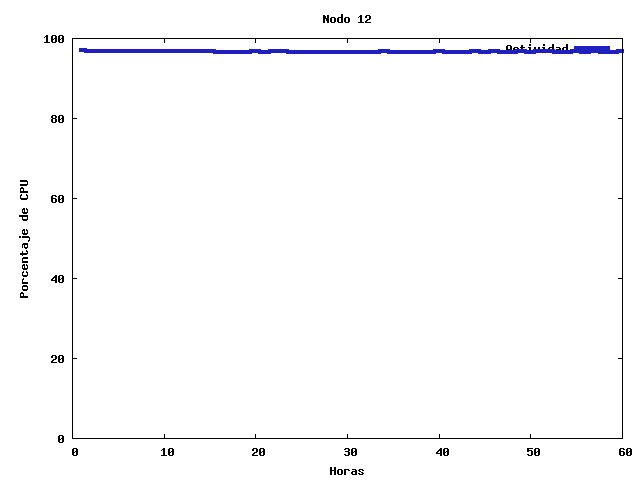
\includegraphics[width=0.9\linewidth]{grafico12.jpg}\\
\caption{Uso de procesadores del duodécimo nodo durante el mes}
\end{figure}

\begin{figure}[htb]
\centering
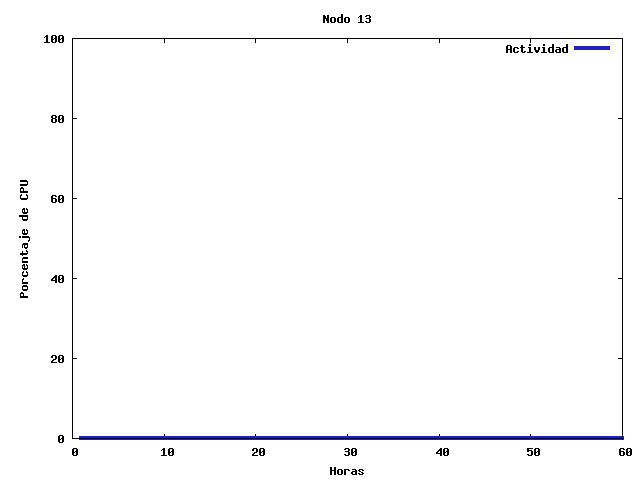
\includegraphics[width=0.9\linewidth]{grafico13.jpg}\\
\caption{Uso de procesadores del nodo 13 durante el mes}
\end{figure}

\begin{figure}[htb]
\centering
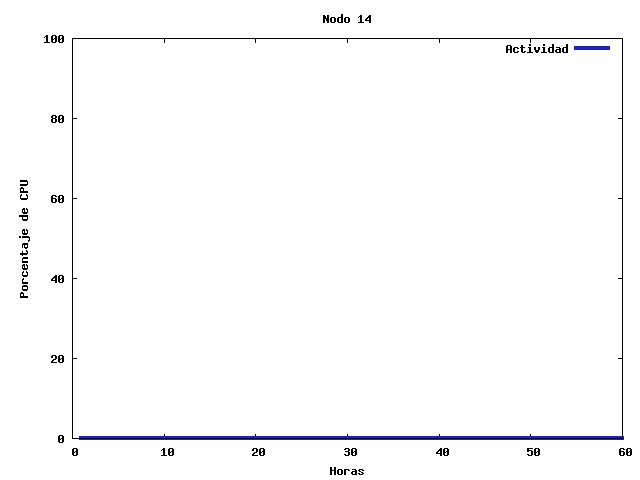
\includegraphics[width=0.9\linewidth]{grafico14.jpg}\\
\caption{Uso de procesadores del nodo 14 durante el mes}
\end{figure}

\begin{figure}[htb]
\centering
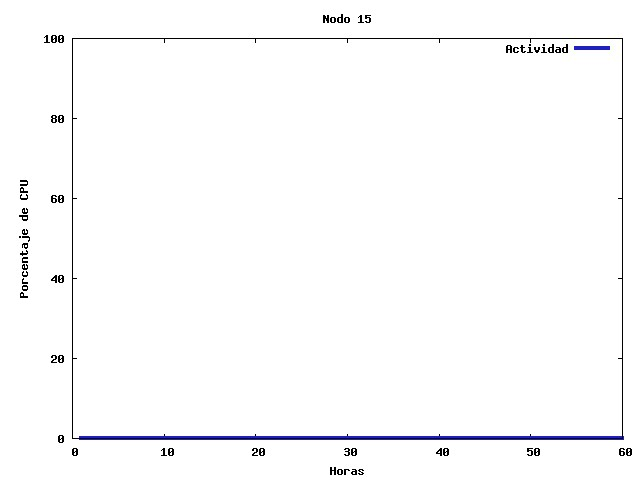
\includegraphics[width=0.9\linewidth]{grafico15.jpg}\\
\caption{Uso de procesadores del nodo 15 durante el mes}
\end{figure}

\begin{figure}[htb]
\centering
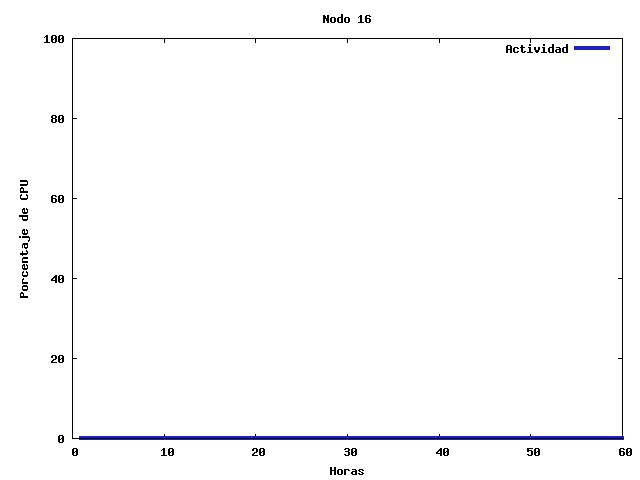
\includegraphics[width=0.9\linewidth]{grafico16.jpg}\\
\caption{Uso de procesadores del nodo 16 durante el mes}
\end{figure}

\textbf{Gráfico de uso de memoria}
\begin{figure}[htb]
\centering
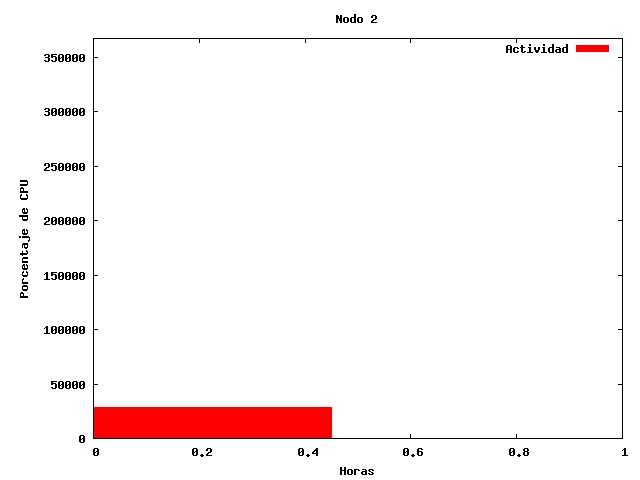
\includegraphics[width=0.9\linewidth]{memoria1.jpg}\\
\caption{Uso de la memoria durante el mes}
\end{figure}

\begin{figure}[htb]
\centering
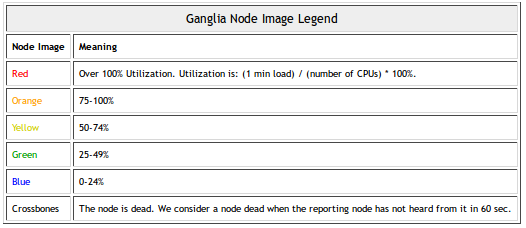
\includegraphics[width=0.9\linewidth]{legend}\\
\end{figure}

%\begin{figure}[htb]
%\begin{multicols}{2}
%\centering
%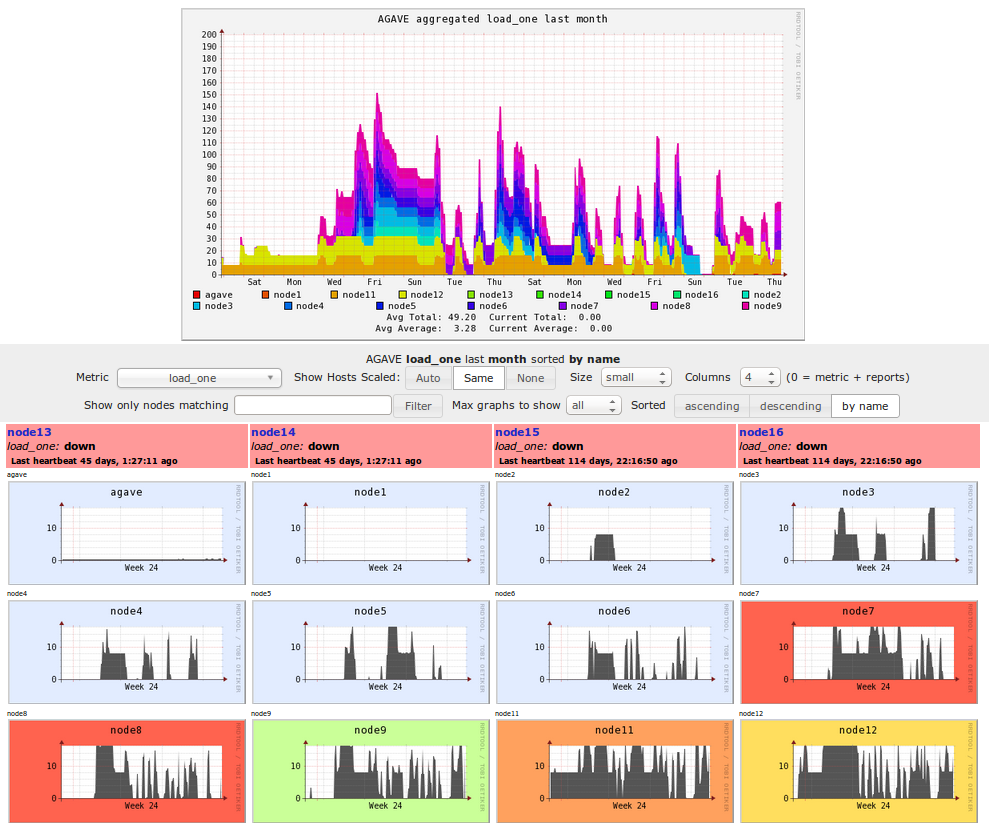
\includegraphics[width=1\linewidth]{estatus_actual}\\
%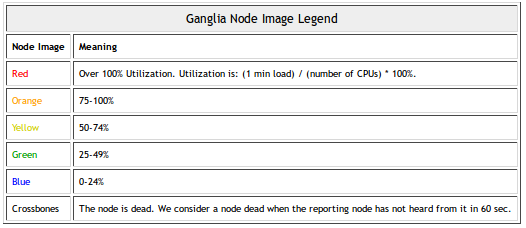
\includegraphics[width=1\linewidth]{legend}\\
%\end{multicols}
%\end{figure}

\end{document}
